\section{Ejercicio 9}

\subsection{Introducción}

Este ejercicio nos pide desarrollar un experimento en cuál se pueda comprobar que el scheduler \textit{SchedEDF} cumple que en un procesador con desalojo y con un único núcleo de procesamiento, si una colección de tareas independientes, cada una caracterizada por su release time y deadline, pueden ser asignadas al procesador de alguna manera que todos los trabajos puedan cumplir su deadline a tiempo, \textit{SchedEDF} va a encontrar una manera de asignarlos de forma que cumplan con sus
deadlines mientras que el resto de los schedulers fallaran.\\
Para simplificar el experimento trataremos el caso en el que todas las tareas tienen un realese time igual a 0, es decir, que todas estaran listas desde el comienzo.\\
Además para que quede visualmente mejor plasmado en los diagramas de \textit{Gantt} correspondientes consideraremos que el scheduler tiene un costo por cambio de contexto igual a 0.

\subsection{Desarrollo}
Para el desarrollo de este experimento se decidió utilizar un lote de 15 tareas cuyos deadlines y ciclos de cpu fueron generados de forma aleatoria.\\
Para esto se implemento un generador de tareas llamado \textit{ej9} el cual se encuentra en la carpeta \textit{generador} del directorio raíz del código fuente.\\
Para correrlo se debe ejecutar el comando \textbf{generador/ej9} $\mathbf{p_1 \; p_2}$ donde $p_1$ y $p_2$ son la cantidad de tareas y el máximo de ciclos de cpu respectivamente.\\
El lote de tareas utilizado se encuentra en la carpeta \textit{tasks} del directorio raíz del código fuente bajo el nombre \textbf{ej9.tsk}.

\subsubsection{Scheduler FCFS}

A continuación veremos como se comporta el scheduler \textit{SchedFCFS} ante el lote de tareas \textbf{ej9.tsk}.\\ 
El mismo asigna el procesador a cada tarea en el orden en el que fueron cargadas y las mantiene en ejecución hasta que terminan.\\
El diagrama de \textit{Gantt} correspondiente es el siguiente:

\begin{figure}[H]
\centering
\makebox[\textwidth][c]{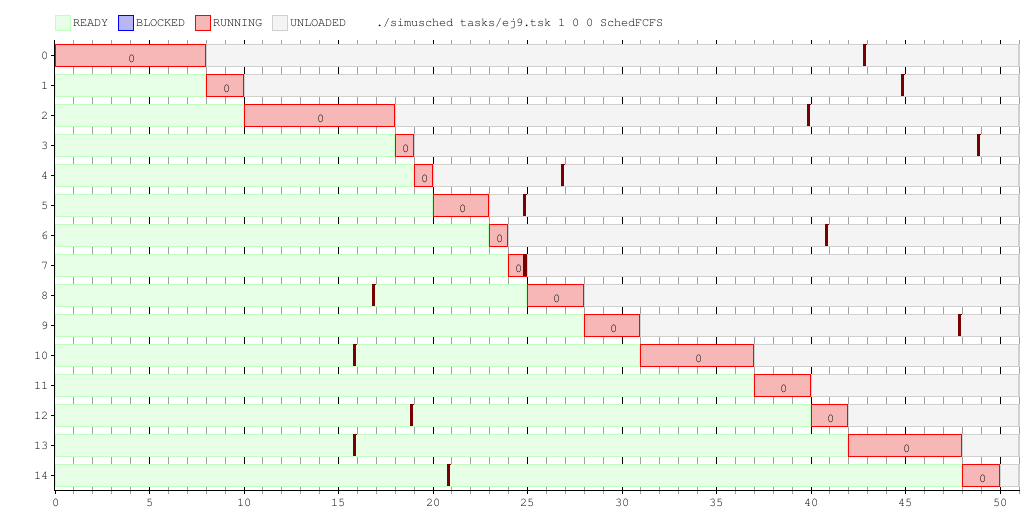
\includegraphics[width=1.2\textwidth]{graphics/ej9-01.png}}%
\caption{Lote de tareas \textbf{ej9.tsk} ejecutándose en \textit{SchedFCFS}}
\label{ej9-fcfs-gantt}
\end{figure}

Como puede observarse en el diagrama de \textit{Gantt} de la figura~\ref{ej9-fcfs-gantt} el scheduler \textit{SchedFCFS} no llega a cumplir con el deadline de todas las tareas.\\

\subsubsection{Scheduler Round Robin}

A continuación veremos como se comporta el scheduler \textit{SchedRR} ante el lote de tareas \textbf{ej9.tsk}.\\ 
El mismo asigna el procesador a cada tarea en el orden en el que fueron cargadas y las mantiene en ejecución hasta que las mismas agotan el quantum asignado, procediendo entonces a ejecutar la próxima tarea en espera.\\
Para el experimento se eligió un quantum igual a 2.\\
El diagrama de \textit{Gantt} correspondiente es el siguiente:

\begin{figure}[H]
\centering
\makebox[\textwidth][c]{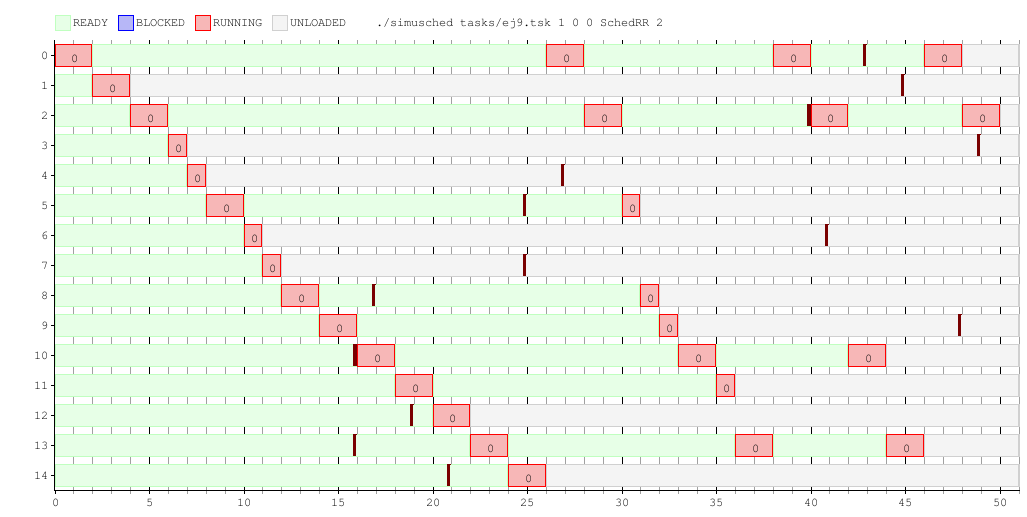
\includegraphics[width=1.2\textwidth]{graphics/ej9-02.png}}%
\caption{Lote de tareas \textbf{ej9.tsk} ejecutándose en \textit{SchedRR}}
\label{ej9-rr-gantt}
\end{figure}

Como puede observarse en el diagrama de \textit{Gantt} de la figura~\ref{ej9-rr-gantt} el scheduler \textit{SchedRR} no llega a cumplir con el deadline de todas las tareas.\\

\subsubsection{Scheduler EDF}

Finalmente veremos como se comporta el scheduler \textit{SchedEDF} ante el lote de tareas \textbf{ej9.tsk}.\\ 
El mismo asigna el procesador a cada tarea según los deadlines de las mismas.\\
El diagrama de \textit{Gantt} correspondiente es el siguiente:

\begin{figure}[H]
\centering
\makebox[\textwidth][c]{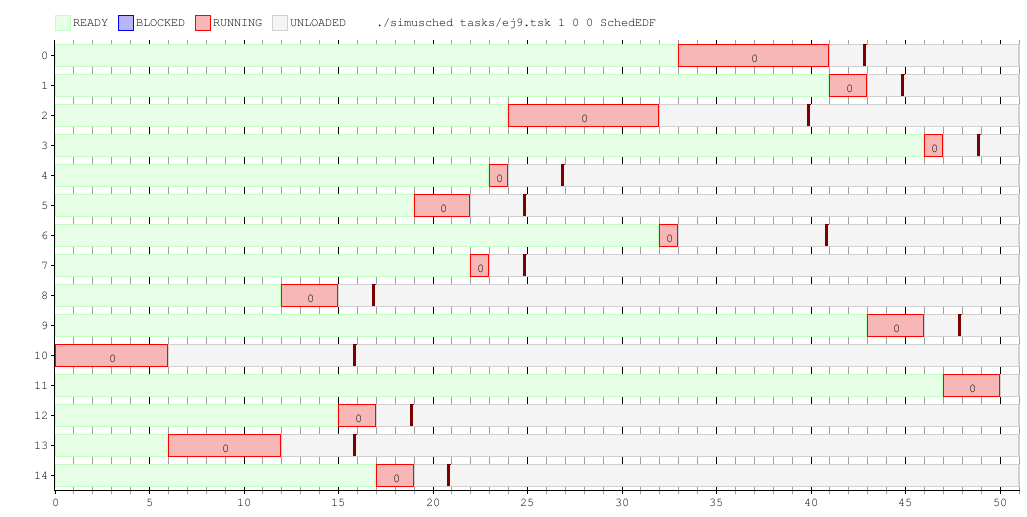
\includegraphics[width=1.2\textwidth]{graphics/ej9-03.png}}%
\caption{Lote de tareas \textbf{ej9.tsk} ejecutándose en \textit{SchedEDF}}
\label{ej9-edf-gantt}
\end{figure}

Como puede observarse en el diagrama de \textit{Gantt} de la figura~\ref{ej9-edf-gantt} el scheduler \textit{SchedEDF} \textbf{si} llega a cumplir con el deadline de todas las tareas.\\

\subsection{Conclusión}
 
Como pudo observarse en los diagramas de \textit{Gantt} de las figuras~\ref{ej9-fcfs-gantt},~\ref{ej9-rr-gantt} y~\ref{ej9-edf-gantt}, en el experimento realizado con un lote de tareas cuyo deadline y ciclos de cpu fueron elegidos de manera aleatoria, solo el scheduler \textit{SchedEDF} logro cumplir con el deadline de todas las tareas.\\
En el presente informe por cuestiones de espacio no exponemos mas lotes de tareas para comparar, pero el interesado puede correr el generador \textbf{ej9} generando lotes de tareas aleatorias y comprobar que lo expuesto mas arriba se sigue cumpliendo.\\
Por lo expuesto concluimos que el scheduler \textit{SchedEDF} \textbf{cumple} que en un procesador con desalojo y con un único núcleo de procesamiento, si una colección de tareas independientes, cada una caracterizada por su release time y deadline, pueden ser asignadas al procesador de alguna manera que todos los trabajos puedan cumplir su deadline a tiempo, \textit{SchedEDF} va a encontrar una manera de asignarlos de forma que cumplan con sus deadlines.
